\subsection{Attention View}
Attention layer is an intermediate layer which gives some sense making information for domain expert to understand what information is generated from previous neural layer and how those information will affect the final prediction.

\begin{figure}[htbp]
	\centering
	\vspace{-2mm}
	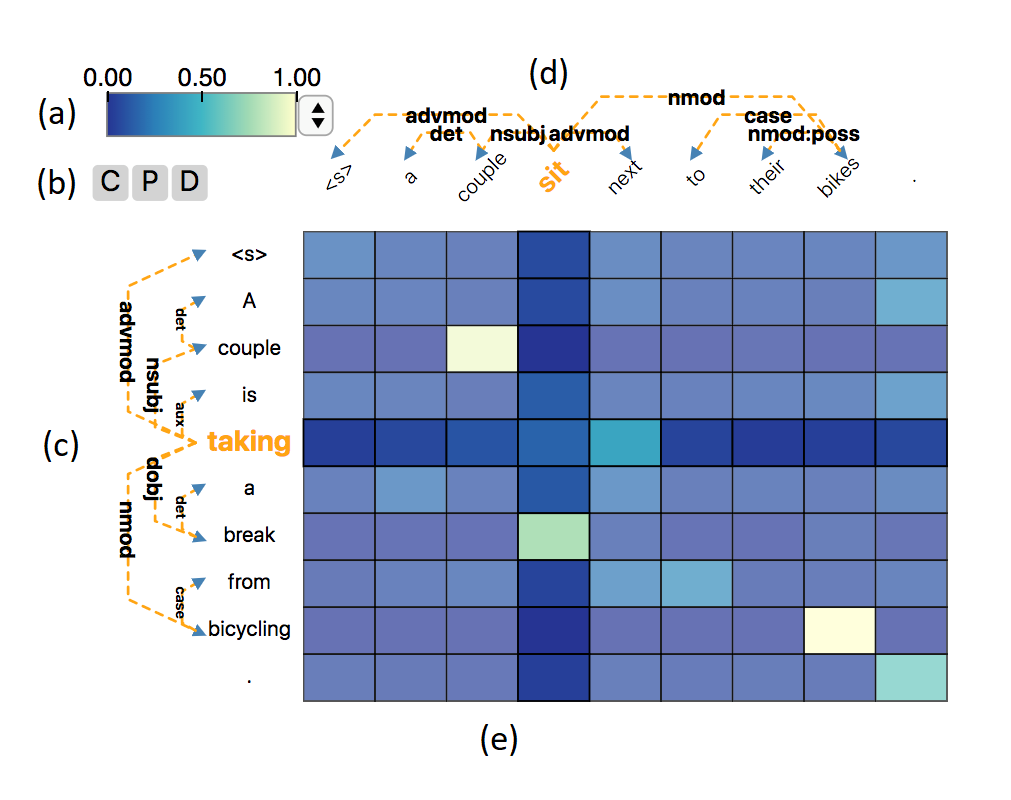
\includegraphics[width=1.0\linewidth]{MatrixAttention}
	\caption{matrix visualize attention}
	\label{fig:MatrixAttention}
\end{figure}


\begin{figure}[htbp]
	\centering
	\vspace{-2mm}
	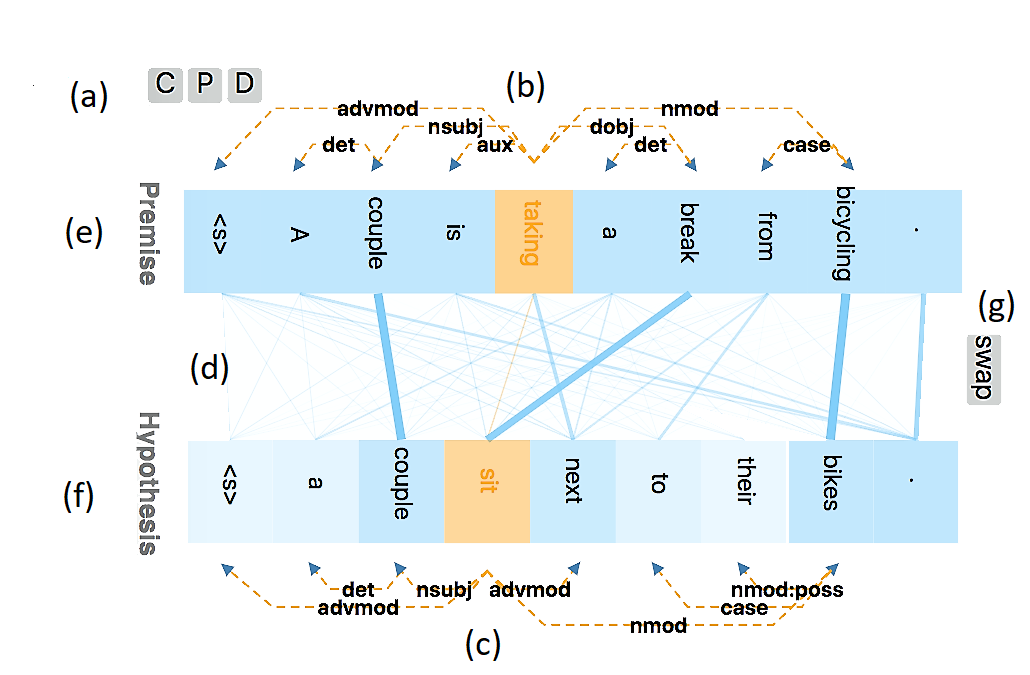
\includegraphics[width=1.0\linewidth]{attentionGraph}
	\caption{bipartite graph visualize attention}
	\label{fig:attentionGraph}
\end{figure}

%\subsubsection{Attention visualization challenges}
\begin{itemize}
	\item Why we need two different visual encoding to visualize attention? bipartite visualization more easier to highlight the 
	\item long sentence, collapse
	\item quickly compare the alignment information with the sentence's linguistic structure.
\end{itemize}


% \subsection{Interpret Attention Via Model Perturbation}
